% Options for packages loaded elsewhere
\PassOptionsToPackage{unicode}{hyperref}
\PassOptionsToPackage{hyphens}{url}
\PassOptionsToPackage{dvipsnames,svgnames,x11names}{xcolor}
\documentclass[
]{article}
\usepackage{xcolor}
\usepackage[margin=22mm]{geometry}
\usepackage{amsmath,amssymb}
\setcounter{secnumdepth}{-\maxdimen} % remove section numbering
\usepackage{iftex}
\ifPDFTeX
  \usepackage[T1]{fontenc}
  \usepackage[utf8]{inputenc}
  \usepackage{textcomp} % provide euro and other symbols
\else % if luatex or xetex
  \usepackage{unicode-math} % this also loads fontspec
  \defaultfontfeatures{Scale=MatchLowercase}
  \defaultfontfeatures[\rmfamily]{Ligatures=TeX,Scale=1}
\fi
\usepackage{lmodern}
\ifPDFTeX\else
  % xetex/luatex font selection
\fi
% Use upquote if available, for straight quotes in verbatim environments
\IfFileExists{upquote.sty}{\usepackage{upquote}}{}
\IfFileExists{microtype.sty}{% use microtype if available
  \usepackage[]{microtype}
  \UseMicrotypeSet[protrusion]{basicmath} % disable protrusion for tt fonts
}{}
\makeatletter
\@ifundefined{KOMAClassName}{% if non-KOMA class
  \IfFileExists{parskip.sty}{%
    \usepackage{parskip}
  }{% else
    \setlength{\parindent}{0pt}
    \setlength{\parskip}{6pt plus 2pt minus 1pt}}
}{% if KOMA class
  \KOMAoptions{parskip=half}}
\makeatother
\usepackage{longtable,booktabs,array}
\newcounter{none} % for unnumbered tables
\usepackage{calc} % for calculating minipage widths
% Correct order of tables after \paragraph or \subparagraph
\usepackage{etoolbox}
\makeatletter
\patchcmd\longtable{\par}{\if@noskipsec\mbox{}\fi\par}{}{}
\makeatother
% Allow footnotes in longtable head/foot
\IfFileExists{footnotehyper.sty}{\usepackage{footnotehyper}}{\usepackage{footnote}}
\makesavenoteenv{longtable}
\usepackage{graphicx}
\makeatletter
\newsavebox\pandoc@box
\newcommand*\pandocbounded[1]{% scales image to fit in text height/width
  \sbox\pandoc@box{#1}%
  \Gscale@div\@tempa{\textheight}{\dimexpr\ht\pandoc@box+\dp\pandoc@box\relax}%
  \Gscale@div\@tempb{\linewidth}{\wd\pandoc@box}%
  \ifdim\@tempb\p@<\@tempa\p@\let\@tempa\@tempb\fi% select the smaller of both
  \ifdim\@tempa\p@<\p@\scalebox{\@tempa}{\usebox\pandoc@box}%
  \else\usebox{\pandoc@box}%
  \fi%
}
% Set default figure placement to htbp
\def\fps@figure{htbp}
\makeatother
\setlength{\emergencystretch}{3em} % prevent overfull lines
\providecommand{\tightlist}{%
  \setlength{\itemsep}{0pt}\setlength{\parskip}{0pt}}
\usepackage{bookmark}
\IfFileExists{xurl.sty}{\usepackage{xurl}}{} % add URL line breaks if available
\urlstyle{same}
\hypersetup{
  colorlinks=true,
  linkcolor={Maroon},
  filecolor={Maroon},
  citecolor={Blue},
  urlcolor={Blue},
  pdfcreator={LaTeX via pandoc}}

\author{}
\date{}

\begin{document}

\section{Paper 16: An Exact Reduction of the Measure Problem --- Finite
Decomposition into Interference Granularity, Event Structure, and
Conditioning}\label{paper-16-an-exact-reduction-of-the-measure-problem-finite-decomposition-into-interference-granularity-event-structure-and-conditioning}

\textbf{Author}: Noriaki Kihara \textbf{Date}: June 12, 2026
\textbf{Version}: v1.0 (final; v0.2 incorporated the 6 mandatory points
of the first review {[}major revision; the entrance examination ---
``report of the selection problem, not a pre-emption of the selection''
--- was passed{]}, v1.0 the points R1--R6 of the second review {[}accept
with minor conditions{]}) \textbf{Series}: Dual Geometry of Wavelength
Space and Frequency Space (Paper 16, sequel to Papers 1--15)

\begin{center}\rule{0.5\linewidth}{0.5pt}\end{center}

\subsection{Abstract}\label{abstract}

The system supplies path amplitudes (transport phases η, Paper 14) with
no free parameters --- the \textbf{raw material} of probability is fully
in stock. What is not yet fixed is the \textbf{aggregation rule} that
bundles the material into probabilities; this is precisely what standard
theory installs as the Born rule, by axiom. This paper does \textbf{not}
select the aggregation rule. Its main result is an \textbf{exact
reduction of the selection problem itself}: (1) \textbf{The historical
proximity 0.0007 was not a meaningful agreement} (Theorem 1): the s=9
twin observable is doubly compressed --- exclusion forces a two-outcome
space, and both measures pile \textasciitilde0.98 onto the dominant
outcome --- collapsing the total-variation distance; in the
three-outcome space at s=11 the divergence \textbf{jumps three orders of
magnitude} to 0.24. A one-line compression lemma (TV
\(=1-\sum\min(P,Q)\le\varepsilon\) when both distributions give the same
dominant outcome mass \(\ge1-\varepsilon\); the tightened form is due to
the reviewer) makes the mechanism exact. (2) \textbf{Structural
divergence} (Theorem 2; stated for the verified domain
\(s\in\{9,11,13\}\), exhaustive): derived (amplitude) measures do not
classicalize to counting measures --- the divergence is persistently
O(0.1--0.9), robust to the convention width of the capacity factor;
\textbf{the two sides share their support (the zeros coincide) and
diverge only in weights}. (3) \textbf{Interference granularity is not
reducible to convention} (Theorem 3): the choice of which alternatives
are summed coherently --- channel-consistent (the historical W) versus
configuration granularity (W′) --- changes values algebraically. The
exact mirror example: \((-3,0,0,0)\) has \(W=0\) exactly under
channel-consistent aggregation yet decays perfectly normally at
configuration granularity (\(W'=768=W'(A)\) exactly). The effect is not
scale-free (it fails at m=2), and at m=4 the \textbf{unit of
cancellation is the channel} --- the mirror does not vanish as a whole
(\(S_+-S_-\neq0\), supporting the parity hypothesis), but channel
(5,7,9) \textbf{cancels by itself} (\(W_A=147456\), \(W_B=0\), \(W'\)
both 3072): per-channel \(W=0\wedge W'>0\) occurs even at even m, so the
supply of granularity divergences is \textbf{richer} than the odd-m
subsequence; moreover \textbf{W′ mirror-equality holds for all channels
at m≥3} (m=2 appears to be a small-s exception). The occurrence
condition has been reduced to \textbf{algebra that is the object of
proof}: the four-value lock \(z^-_K/z^+_K\in\{0,\infty,\pm1\}\) (all 36
configurations, zero exceptions; exclusive families weigh equally,
384=384). (4) \textbf{Conditioning demands the branch-channel stratum}
(Theorem 4): the twin measure is a function of the parent pair's
relation class; the check that could have failed is that pairs
indistinguishable by intensity fringes (the sign of dot) have
\textbf{different} P(X) --- the measure cannot be supported on strata
1--2 of the readout hierarchy 11⊂13⊂21 (Paper 13, Theorem 3) and
requires stratum 3. (5) \textbf{Event structure is exactly one bit}:
one-shot (merged-key) versus sequential (split-key) translates, via the
record principle, into interference granularity; the historical counting
dichotomy is its phase-free shadow --- the 2×2 table is numerically
complete. (6) \textbf{Main theorem} (Theorem 6, a classification within
the family): the inventory-defined candidates organize without
duplication into the product of three independent axes --- granularity ×
event-structure bit × conditioning --- each axis independently changing
the measure (with explicit examples); no claim is made that candidates
outside the family cannot exist. The decision experiments are
\textbf{computable inside the model} (decision table, §9; items m=4 and
ι executed before publication --- Supplement 84; m=5@s31 honestly
registered as open, the load-bearing point for the Born question). Under
this reduction the Born rule has the status of an \textbf{effective law
to be merged with in a suitable limit}, with the three-part acceptance
criterion \textbf{convergence, suppression (statistical censorship
\textasciitilde1/√N), and prediction}. No physical identification is
made.

\begin{center}\rule{0.5\linewidth}{0.5pt}\end{center}

\subsection{1. Introduction}\label{introduction}

\subsubsection{1.1 The question, and why this paper does not
select}\label{the-question-and-why-this-paper-does-not-select}

Papers 5--15 established states, conservation, time, position, phases,
and coordinates as theorems or machine verifications. What remains is
the rule that turns the set of amplitudes η into \textbf{probability}
--- which alternatives to add coherently (granularity), what to
condition on, and under which event structure to read. Standard theory
settles this with one axiom: the Born rule. The present system has the
opposite problem: aggregation candidates are \textbf{over-derivable} ---
sequential and batch counting, channel-consistent and
configuration-granularity amplitudes, one-shot and sequential joint
amplitudes are all definable from stock, and they genuinely differ at
finite s. The honest deliverable at this stage is therefore not a
verdict but an \textbf{exact reduction of the selection problem with
internally computable decision experiments}. That is this paper.

\subsubsection{1.2 What is not claimed}\label{what-is-not-claimed}

\begin{enumerate}
\def\labelenumi{(\roman{enumi})}
\tightlist
\item
  Selection of the aggregation rule (no result here depends on it). (ii)
  A derivation of the Born rule (only its status is organized --- §10).
  (iii) The reality of deviations (only the location of their
  structure). (iv) No physical identification.
\end{enumerate}

\subsection{2. Definitions (the measure family at general
s)}\label{definitions-the-measure-family-at-general-s}

For twins \((s,s)\) (capacities \(c(m)=|SH[m]|\); channels =
\texttt{all\_finals(s)}):

\begin{itemize}
\tightlist
\item
  \textbf{D1 (sequential counting)}: first-channel probability ∝
  configuration count on the remaining lattice; the second is the
  conditional update. Well-definedness rests on the lemma that
  conditional counts depend only on per-shell occupancies (products of
  binomial capacities).
\item
  \textbf{D2 (batch counting)}: equal weight on joint final
  configurations.
\item
  \textbf{D3 (derived twin)}:
  \(P\propto \mathrm{mult}\cdot W_{F_1}W_{F_2}\cdot[\)joint capacity
  compatibility\(]\), with \(W_F=|z_F|^2\) the channel-consistent
  amplitude under the canonical counting of Paper 14, Theorem 5.
\item
  \textbf{W′ (configuration granularity)}: \(W'_F=\sum_K|z_K|^2\)
  (square per final configuration \(K\), then sum).
\item
  \textbf{D4 (tracking observable)}:
  \(\Delta(s)=\mathrm{TV}(\text{D3},\text{D1})\); \(\Delta'(s)\) is the
  W′ version.
\end{itemize}

Anchors (s=9), all exactly reproduced: sequential 396/403, batch 60/61,
derived 0.98195, \(\Delta(9)=0.00068\), single decay 24/31.

\subsection{3. Theorem 1: the identity of 0.0007 is two-outcome
compression}\label{theorem-1-the-identity-of-0.0007-is-two-outcome-compression}

\textbf{Compression lemma (one line)}: if two probability distributions
both give the same dominant outcome mass \(\ge1-\varepsilon\), then
\(\mathrm{TV}=1-\sum\min(P,Q)\le\varepsilon\) (the tightened form is due
to the reviewer). In the s=9 twin, (i) exclusion (uniqueness of the
origin cell) forces a two-outcome space, and (ii) both measures
concentrate \textasciitilde0.98 on the dominant outcome
(\(\varepsilon\approx0.018\)) --- this double compression had crushed
the TV (Fig. 1a). When the three-outcome space opens at s=11,
\(\Delta(11)=0.24136\) --- a \textbf{three-order jump} (Fig. 1b).
Corroboration: at the single-decay level even s=9 shows 0.774 vs 0.965;
sector B has \(\Delta_B(9)=0.030\). \textbf{The proximity of 0.98195 and
0.98263 was an accident of s=9 and sector A}; the historical
significance attached to it is corrected here (the values themselves
stand).

\subsection{4. Theorem 2: structural divergence (no
classicalization)}\label{theorem-2-structural-divergence-no-classicalization}

\textbf{Verified domain made explicit}: this theorem is a statement at
the exhaustive level for \(s\in\{9,11,13\}\) (a three-point series).
Over this series \(\Delta(s)\) runs 0.0007 → 0.24 → up to 0.90 (strong
parent-type and sector dependence; Fig. 2). The internal width of the
counting side (TV(sequential, batch)) is always an order of magnitude
smaller. The graded variant of the capacity factor does not remove the
O(0.1) divergence --- \textbf{robust to convention width}. The
independent general-s observable D(s) likewise fails to shrink
(0.135→0.140→0.185). Meanwhile, \textbf{support coincidence}:
capacity-impossible channels and amplitude-zero channels coincide
bidirectionally at s=9/11/13 (only the \((1,1,s{-}2)\) type) --- the two
sides \textbf{share their zeros and diverge only in weights}.

\subsection{5. Theorem 3: the non-conventionality of interference
granularity}\label{theorem-3-the-non-conventionality-of-interference-granularity}

\textbf{Internal definition (convention)}: in this series a
``convention'' is a choice of presentation that does not change the
bookkeeping values (e.g., the diagonal and branch treatments --- the
granularity audit of Paper 14, Theorem 5). The choice between the
channel-consistent sum (historical W: coherent across
record-distinguishable final configurations) and configuration
granularity (W′: square per configuration) is \textbf{not} a convention
in this sense --- it splits values algebraically (Fig. 3a):

{\def\LTcaptype{none} % do not increment counter
\begin{longtable}[]{@{}lll@{}}
\toprule\noalign{}
Parent & W (channel-consistent) & W′ (configuration granularity) \\
\midrule\noalign{}
\endhead
\bottomrule\noalign{}
\endlastfoot
\((+3,0,0,0)\)@13 & 9216 & 768 (30 configurations) \\
\((-3,0,0,0)\)@13 (mirror) & \textbf{0 (exact)} & \textbf{768 = W′(A)
exact} \\
\end{longtable}
}

The mirror parent decays perfectly normally at configuration
granularity; only the channel-consistent aggregate bends a healthy
distribution to exact zero. Moreover (the m=4 execution of Supplement
84, propagated into this section --- R1): (i) the cancellation is
\textbf{not scale-free} (at m=2, \(W(B)=32\neq0\) and W′ also differ)
--- the occurrence condition depends on m. \textbf{At m=4 (s=21) the
unit of cancellation turns out to be the channel}: the mirror does not
vanish as a whole (\(S_+-S_-\neq0\), supporting the parity hypothesis),
but \textbf{channel (5,7,9) cancels by itself} (\(W_A=147456\),
\(W_B=0\), \(W'\) both 3072) --- per-channel \(W=0\wedge W'>0\) occurs
even at even m, so the supply of granularity divergences is
\textbf{richer} than the odd-m subsequence. Also, \textbf{W′
mirror-equality holds for all channels at m≥3} (the m=2 discrepancy
appears to be a small-s exception). (ii) The m-dependence is reduced by
the \textbf{mirror-flip lemma} \(\eta_B/\eta_A=-i(-1)^{\sigma_0}\) (394
paths, zero exceptions) to the vanishing of a \textbf{σ-parity indicator
sum} \(S_+=S_-\), and at configuration level is pinned to the
\textbf{four-value lock} \(z^-_K/z^+_K\in\{0,\infty,+1,-1\}\) (all 36
configurations at m=3: 12+12+6+6, zero exceptions; exclusive families
weigh equally, 384=384; Fig. 3b) --- algebra that is \textbf{the object
of proof}. (iii) Sector (holonomy) dependence nearly vanishes at
configuration granularity (\(W'\) A≈B) --- \textbf{holonomy information
is localized in the relative phases between configurations}.

\subsection{6. Theorem 4: conditioning demands the branch-channel
stratum}\label{theorem-4-conditioning-demands-the-branch-channel-stratum}

\textbf{Terminology note}: the ``A/B'' of mirror pairs in this paper
(parents \(\pm m\)) and the ``A/B'' holonomy classes of Paper 14, §5 are
\textbf{distinct} --- beware when reading both.

The joint amplitude of twins depends strongly on the relative
configuration of the parent pair (including completely cancelling
pairs). The three-stratum discipline (review \#4):
\textbf{class-constancy (s=9 sector A, 23 pairs, all 9 classes, zero
exceptions) is ① true by construction} --- the invariant classes are the
exact orbit classification (B₄×swap), so constancy follows from the
equivariance of the machinery and has no refutation power (a consistency
check). \textbf{The check that could have failed (③) --- the fang of
this section --- is this}: pairs with dot=±1, indistinguishable by
intensity fringes, have \textbf{different} P(X) (0.972 vs 0.994 --- they
could have been equal). Hence the measure cannot be supported on strata
1--2 of the readout hierarchy 11⊂13⊂21 (Paper 13, Theorem 3) and
\textbf{requires stratum 3 (branch channels)}. The principle
``interference granularity = record distinguishability'' holds only with
the stratum made explicit. The floor (pairs with disjoint axis supports
= the configuration-granularity value 0.96644) is also ③: it agreed with
the granularity audit independently.

\subsection{7. Event structure: exactly one
bit}\label{event-structure-exactly-one-bit}

One-shot (no intermediate append → outcome = merged occupied set →
splits indistinguishable → coherent across splits) versus sequential
(the first append fixes the split) --- the record principle translates
this single bit into interference granularity. The historical counting
dichotomy (batch 60/61, sequential 396/403) is its phase-free shadow;
everything fits the 2×2 table (numerically complete):

{\def\LTcaptype{none} % do not increment counter
\begin{longtable}[]{@{}
  >{\raggedright\arraybackslash}p{(\linewidth - 4\tabcolsep) * \real{0.3333}}
  >{\raggedright\arraybackslash}p{(\linewidth - 4\tabcolsep) * \real{0.3333}}
  >{\raggedright\arraybackslash}p{(\linewidth - 4\tabcolsep) * \real{0.3333}}@{}}
\toprule\noalign{}
\begin{minipage}[b]{\linewidth}\raggedright
\end{minipage} & \begin{minipage}[b]{\linewidth}\raggedright
one-shot
\end{minipage} & \begin{minipage}[b]{\linewidth}\raggedright
sequential
\end{minipage} \\
\midrule\noalign{}
\endhead
\bottomrule\noalign{}
\endlastfoot
counting & 0.98361 & 0.98263 \\
amplitude & pair-dependent: mean 0.989, range {[}0.966, 1.000{]} +
completely cancelling pairs (surviving both keyings) & pair-dependent:
mean 0.781, range {[}0, 1{]} \\
\end{longtable}
}

The amplitude side retains pair dependence under either event structure
--- conditioning (§6) is an inseparable component.

\subsection{8. The proven cancellation theorems (with scope
qualifications)}\label{the-proven-cancellation-theorems-with-scope-qualifications}

This line of inquiry has proven the exact cancellations on
channel-consistent sums in the \textbf{style of involutions and
indicator sums}: (i) \(\Sigma\eta^2=0\) (the piecewise involution σ**
--- completeness, no fixed points, \(\eta\to\pm i\eta\); \textbf{at the
exhaustive level of s=9}). (ii) A1 (\(\Sigma i^{\delta_1}=0\)) --- the
shell-level involution \(x\leftrightarrow x\mp2\) (borrow ↔ lend). (iii)
B2 (\(Z_4\) equidistribution of sin-branch counts) --- torsor residues
(4-solution orbits are complete residue systems) × stage factorization;
\textbf{based on the fiber structure of the 531 path set; the 333 final
is not equidistributed}. (iv) The mirror-flip lemma and the
indicator-sum reduction (§5). These are the \textbf{internal structure}
of one aggregation candidate (channel-consistent sums), complementary to
the adjudication of its status (this reduction).

\subsection{9. Main theorem (classification of the candidate family) and
the decision
table}\label{main-theorem-classification-of-the-candidate-family-and-the-decision-table}

\begin{quote}
\textbf{Theorem 6 (classification within the family --- the main
theorem)}: for the inventory-defined family of aggregation candidates
--- \{counting D1/D2; amplitude channel-consistent W; configuration
granularity W′\} × \{one-shot, sequential\} × \{with/without
relation-class conditioning\}: (i) any two candidates of the family
\textbf{can} differ by total variation O(0.1) at finite \(s\)
(exhaustive at \(s\le13\)) --- they are genuinely distinct measures.
(ii) All candidates share support coincidence (§4) and canonical
counting (Paper 14, Theorem 5). (iii) \textbf{The independently defined
candidates organize without duplication into this product, and each of
the three axes is independent} --- every axis has an explicit example
where changing it alone changes the measure (granularity: the mirror
\(W=0\wedge W'>0\); event structure: 0.98361 vs 0.98263, and
joint-amplitude means 0.989 vs 0.781; conditioning: the dot=±1
inequality). This is a \textbf{classification theorem within the
family}; no universal claim is made that candidates outside the family
cannot exist (limitation per review \#1; the non-trivial content of
(iii) is the duplication-free organization and the independence of the
axes --- R2).
\end{quote}

\subsubsection{Decision table (experiments computable inside the
model)}\label{decision-table-experiments-computable-inside-the-model}

{\def\LTcaptype{none} % do not increment counter
\begin{longtable}[]{@{}
  >{\raggedright\arraybackslash}p{(\linewidth - 6\tabcolsep) * \real{0.2500}}
  >{\raggedright\arraybackslash}p{(\linewidth - 6\tabcolsep) * \real{0.2500}}
  >{\raggedright\arraybackslash}p{(\linewidth - 6\tabcolsep) * \real{0.2500}}
  >{\raggedright\arraybackslash}p{(\linewidth - 6\tabcolsep) * \real{0.2500}}@{}}
\toprule\noalign{}
\begin{minipage}[b]{\linewidth}\raggedright
\#
\end{minipage} & \begin{minipage}[b]{\linewidth}\raggedright
Experiment
\end{minipage} & \begin{minipage}[b]{\linewidth}\raggedright
What it decides
\end{minipage} & \begin{minipage}[b]{\linewidth}\raggedright
Status
\end{minipage} \\
\midrule\noalign{}
\endhead
\bottomrule\noalign{}
\endlastfoot
1 & Parity hypothesis: m odd ⟺ \(S_+=S_-\) & the occurrence condition of
mirror cancellation & \textbf{m=4 executed (Suppl. 84): supported} ---
\(S_+-S_-\neq0\); however channel (5,7,9) cancels even at even m (the
unit refines to per-channel indicator sums). \textbf{W′ mirror-equality
is generic for m≥3} (all channels exact). m=5@s31 remains (the Born
load-bearing point) \\
2 & Mutual convergence of candidates at large s (\(\Delta/\Delta'\)
series, per granularity) & whether measure selection matters only in the
deep discrete regime or everywhere & open \\
3 & The ι construction (axis-0 branch flip of the hidden vx) & proof
component of the four-value lock & \textbf{executed (Suppl. 84):
complete at m=3} --- configuration-preserving, σ-flipping, 384/384;
multiplier exactly ±1 (192/192). \textbf{At m=2 the closure of the path
set breaks (2/10)} --- the structural address of ``why odd m'' =
ι-closure. Remaining: the distribution law of the multiplier within
configurations \\
4 & Gauge independence (invariance of the measure under marking and
orientations) & the falsifiable content of principle v2 & open \\
5 & Comparison of isomorphic pairs in the unsaturated regime at s=11 &
whether the dot=±2 equality is saturation or an extra symmetry & open \\
\end{longtable}
}

\subsection{10. The status of the Born rule and the acceptance
criterion}\label{the-status-of-the-born-rule-and-the-acceptance-criterion}

Under this reduction, the Born rule is not ``an exact target to
reproduce'' but an \textbf{effective law to be merged with within limits
and censorship precision}. The acceptance criterion is the triple:
\textbf{convergence} (the selected measure merges with Born in a
suitable limit --- the limit map itself is a construction task),
\textbf{suppression} (in domains corresponding to verified regimes,
deviations below \textbf{statistical censorship} \textasciitilde1/√N ---
the statistical version of Paper 15's censorship quantum), and
\textbf{prediction} (verifiable structure in the deep discrete regime
--- granularity, parity, quantization). The floor is secured: if
internal principles do not decide, one aggregation rule can be installed
as a postulate, placing the axiom count level with standard theory
(never below). The upside is that the record principle (the
branch-channel stratum) fixes the aggregation uniquely --- then an
analogue of the Born rule becomes a theorem.

\subsection{11. Honest limits}\label{honest-limits}

\begin{enumerate}
\def\labelenumi{\arabic{enumi}.}
\tightlist
\item
  \textbf{No selection has been made} (§1.2) --- the reduction is
  preparation for selection; which of the three components is fixed
  first depends on executing the decision table.
\item
  The numerical series are exhaustive facts at s≤13 (partly s=11).
  Large-s behavior is decision-table item 2.
\item
  The parent-pair sweep of joint amplitudes is s=9, sector A (23 pairs).
  Sweeps at s≥11 and mixed-sector pairs are unexecuted.
\item
  The four-value lock and the weight pairing are exhaustive facts at m=3
  (the proof is in progress along decision-table item 3).
\item
  No physical identification is made.
\end{enumerate}

\subsection{Figures}\label{figures}

\begin{itemize}
\tightlist
\item
  \textbf{Figure 1} (\texttt{paper16\_fig1\_compression.png}):
  two-outcome compression --- joint distributions at s=9 (2 outcomes,
  Δ=0.00068) and s=11 (3 outcomes, Δ=0.24136)
\end{itemize}

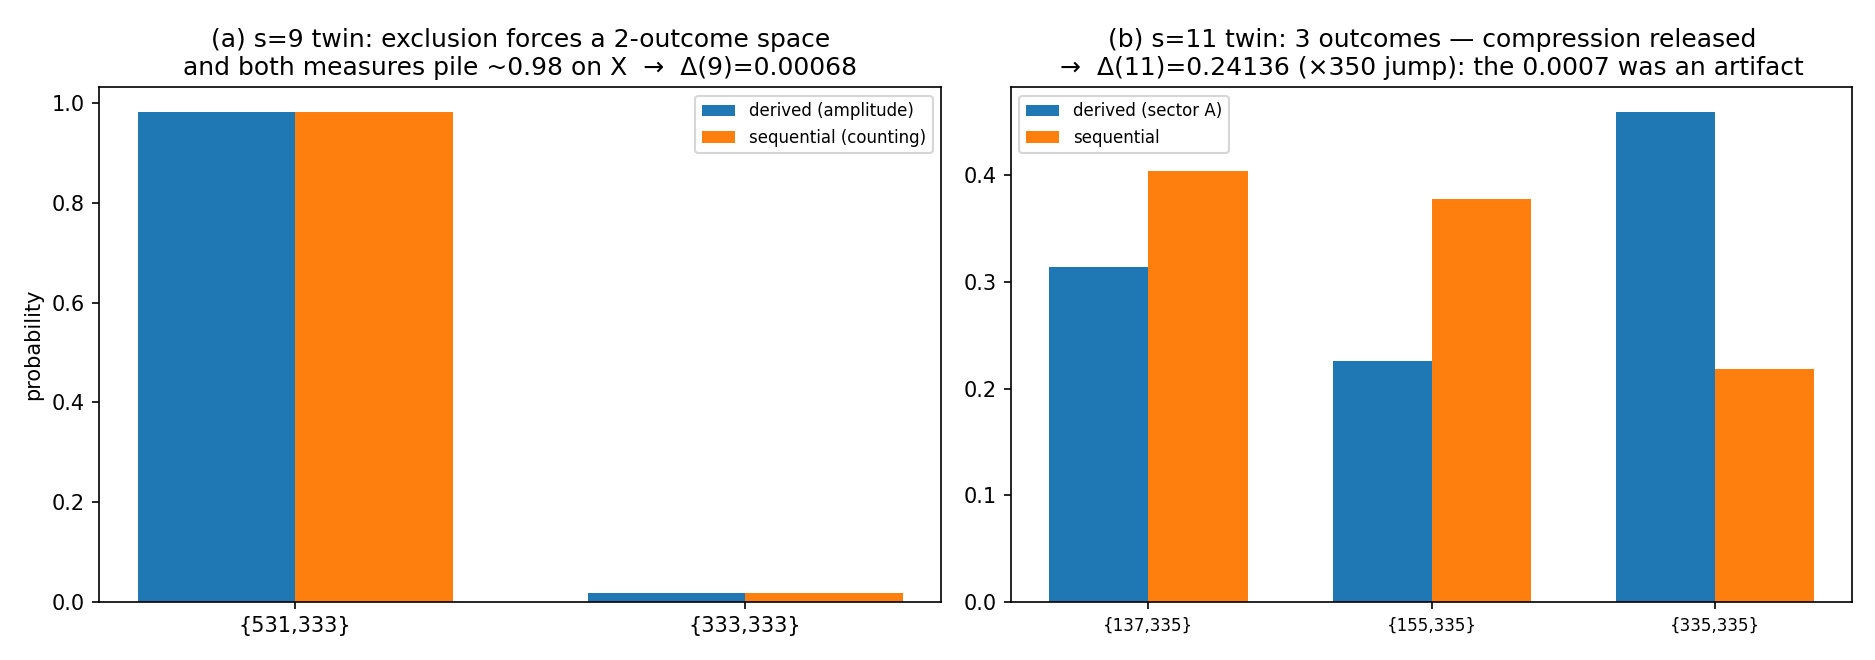
\includegraphics[width=1\linewidth,height=\textheight,keepaspectratio]{paper16_fig1_compression.png}
- \textbf{Figure 2} (\texttt{paper16\_fig2\_divergence.png}): the
divergence landscape --- the Δ(s) series over all parent types, and
configuration-granularity Δ′ (collapse of sector dependence)

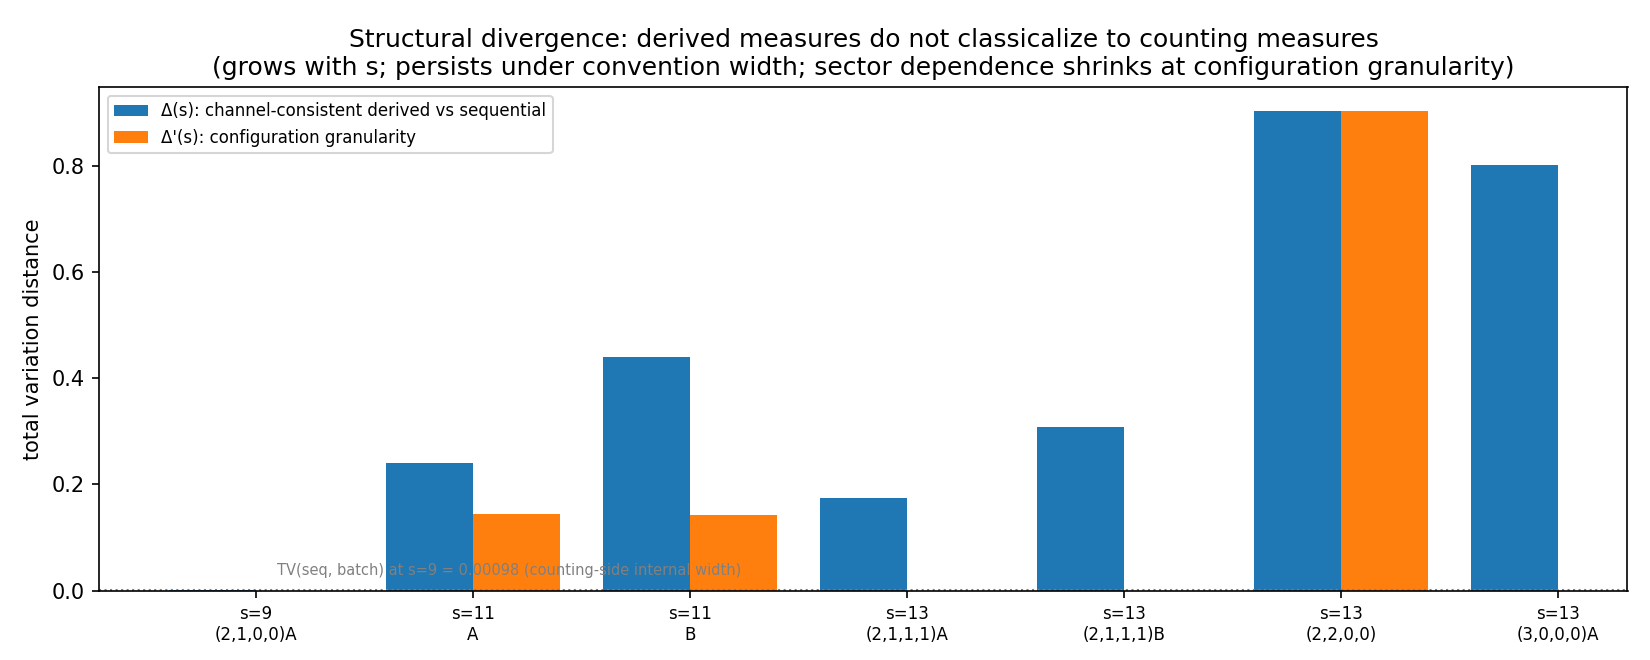
\includegraphics[width=1\linewidth,height=\textheight,keepaspectratio]{paper16_fig2_divergence.png}
- \textbf{Figure 3} (\texttt{paper16\_fig3\_granularity.png}):
non-conventionality of granularity --- the mirror-cancellation m-series
(absent at m=2; full at m=3; per-channel (5,7,9) at m=4) and W′
mirror-equality (m≥3); the four-value lock 12+12+6+6 and the weight
pairing 384=384

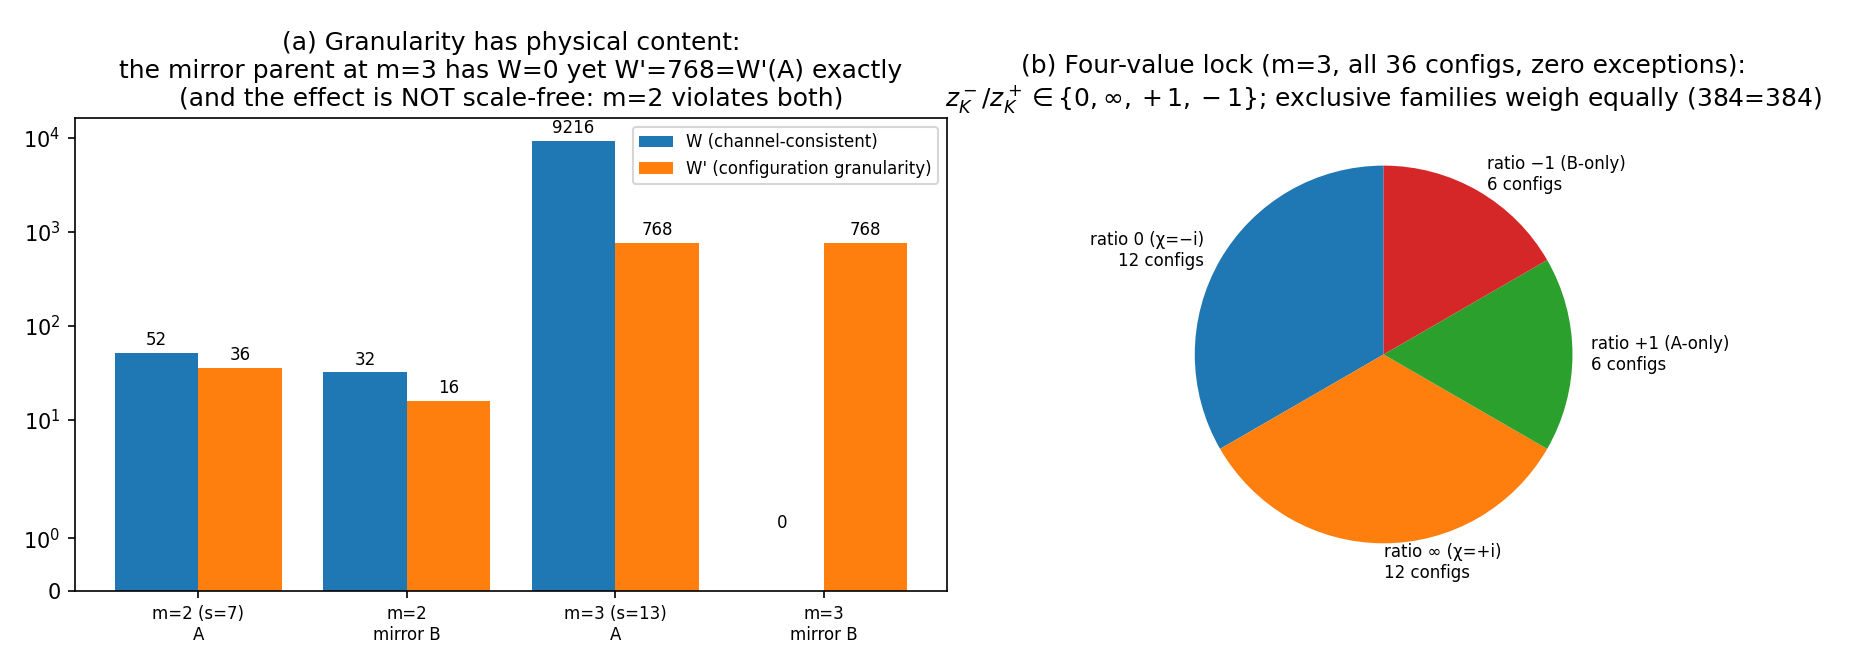
\includegraphics[width=1\linewidth,height=\textheight,keepaspectratio]{paper16_fig3_granularity.png}

All figures are presentations of machine-verified values (no
schematics).

\subsection{Appendix A: Verification summary (labels: ① true by
construction / ② theorem + confirmation / ③ check that could have
failed)}\label{appendix-a-verification-summary-labels-ux2460-true-by-construction-ux2461-theorem-confirmation-ux2462-check-that-could-have-failed}

{\def\LTcaptype{none} % do not increment counter
\begin{longtable}[]{@{}
  >{\raggedright\arraybackslash}p{(\linewidth - 8\tabcolsep) * \real{0.2000}}
  >{\raggedright\arraybackslash}p{(\linewidth - 8\tabcolsep) * \real{0.2000}}
  >{\raggedright\arraybackslash}p{(\linewidth - 8\tabcolsep) * \real{0.2000}}
  >{\raggedright\arraybackslash}p{(\linewidth - 8\tabcolsep) * \real{0.2000}}
  >{\raggedright\arraybackslash}p{(\linewidth - 8\tabcolsep) * \real{0.2000}}@{}}
\toprule\noalign{}
\begin{minipage}[b]{\linewidth}\raggedright
Claim
\end{minipage} & \begin{minipage}[b]{\linewidth}\raggedright
Label
\end{minipage} & \begin{minipage}[b]{\linewidth}\raggedright
Verification
\end{minipage} & \begin{minipage}[b]{\linewidth}\raggedright
Method
\end{minipage} & \begin{minipage}[b]{\linewidth}\raggedright
Script
\end{minipage} \\
\midrule\noalign{}
\endhead
\bottomrule\noalign{}
\endlastfoot
Anchor reproduction & ③ & all points & exact (rational arithmetic) &
supplement73\_handoff\_execution.py \\
Δ(9/11/13), all parent types & ③ & table (Fig. 2) & exhaustive & same \\
Support coincidence & ③ & s=9/11/13 bidirectional & exhaustive & same \\
Graded convention width & ③ & s=9/11/13 & exhaustive & same \\
Mirror parent W=0∧W′ / m=2,4 & ③ & m=1--4 & exhaustive &
supplement75/79/84 scripts \\
Class constancy & \textbf{① (consequence of equivariance --- consistency
check)} & 23 pairs × 9 classes & exhaustive &
supplement75\_granularity\_execution.py \\
Fringe-class test (stratum-3 requirement) & \textbf{③ (the fang)} &
dot=±1 inequality & exhaustive & suppl. 75/77 \\
2×2 table (incl.~A\_seq) & ③ & complete & exhaustive / sweep &
supplement75\_granularity\_execution.py \\
Cancellation theorems (σ**, A1, B2) & ② (involution constructions =
proofs) & s=9 level & exhaustive + involutions & supplement69/70/71
scripts \\
Mirror-flip lemma, indicator-sum reduction & ② (three-line arithmetic) &
394 paths, 0 exceptions & exhaustive &
supplement81\_mirror\_lemma\_check.py \\
Four-value lock, weight pairing & ③ (ι is upgrading it toward ②) & 36
configs, 0 exceptions; 384=384 & exhaustive & suppl. 83 (verification
record), suppl. 84 (ι) \\
\end{longtable}
}

\begin{center}\rule{0.5\linewidth}{0.5pt}\end{center}

\textbf{Acknowledgments / history}: verification was carried out under
the two-party independent verification protocol of Claude Code (local
machine verification) and claude.ai (independent re-computation;
proposal and mutual correction of several propositions). Source
material: Supplements 68--84 (June 12, 2026; suppl. 83 = the
four-value-lock verification record, suppl. 84 = the m=4 and ι
executions). In the course of this line, predictions were refuted
(scale-freeness), explanations corrected (σ₀ constancy), and definitions
reconciled (the three fringe strata) across seven exchanges between the
two parties --- the reliability of the reduction rests on this history
of mutual correction. v0.2: 6 mandatory points of the first review.
v1.0: points R1--R6 of the second review --- propagation of Supplement
84 into §5 and Fig. 3, the non-trivialized Theorem 6(iii), the
compression lemma, distribution ranges, terminology note.

No physical identification is made.

\end{document}
